\section{41 - MAT - AG 4.1, AN 1.1, FA 5.1  - Krippenstein/five fingers - Matura 2013/14 2. Nebentermin}

\begin{langesbeispiel} \item[0] %PUNKTE DES BEISPIELS
				Die Dachsteinseilbahn erschlie�t vom ober�sterreichischen Ort Obertraun aus den n�rdlichen Teil des Dachsteinmassivs. Die Dachsteinseilbahn besteht aus drei Teilstrecken. Die erste Teilstrecke auf die Sch�nbergalm ist bereits seit 1951 in Betrieb. Die zweite Teilstrecke f�hrt von der Sch�nbergalm zum Krippenstein. Von dort aus ist die Aussichtsplattform \textit{five fingers} durch einen Fu�weg erreichbar. Die dritte Teilstrecke f�hrt vom Krippenstein weiter zur Gjaidalm. 
				
				Bei den folgenden Aufgabenstellungen werden Orte als Punkte modelliert. 

\subsection{Aufgabenstellung:}
\begin{enumerate}
	\item Die Bergstation Krippenstein $K_1$ und die Sch�nbergalm $S$ sind durch eine Seilbahn verbunden. Der Verlauf des Tragseils wird, wie in der nebenstehenden Abbildung dargestellt, modelliert. Dabei werden $x$ und $y$ in Metern gemessen.
	
	
	\begin{center}
	\resizebox{0.5\linewidth}{!}{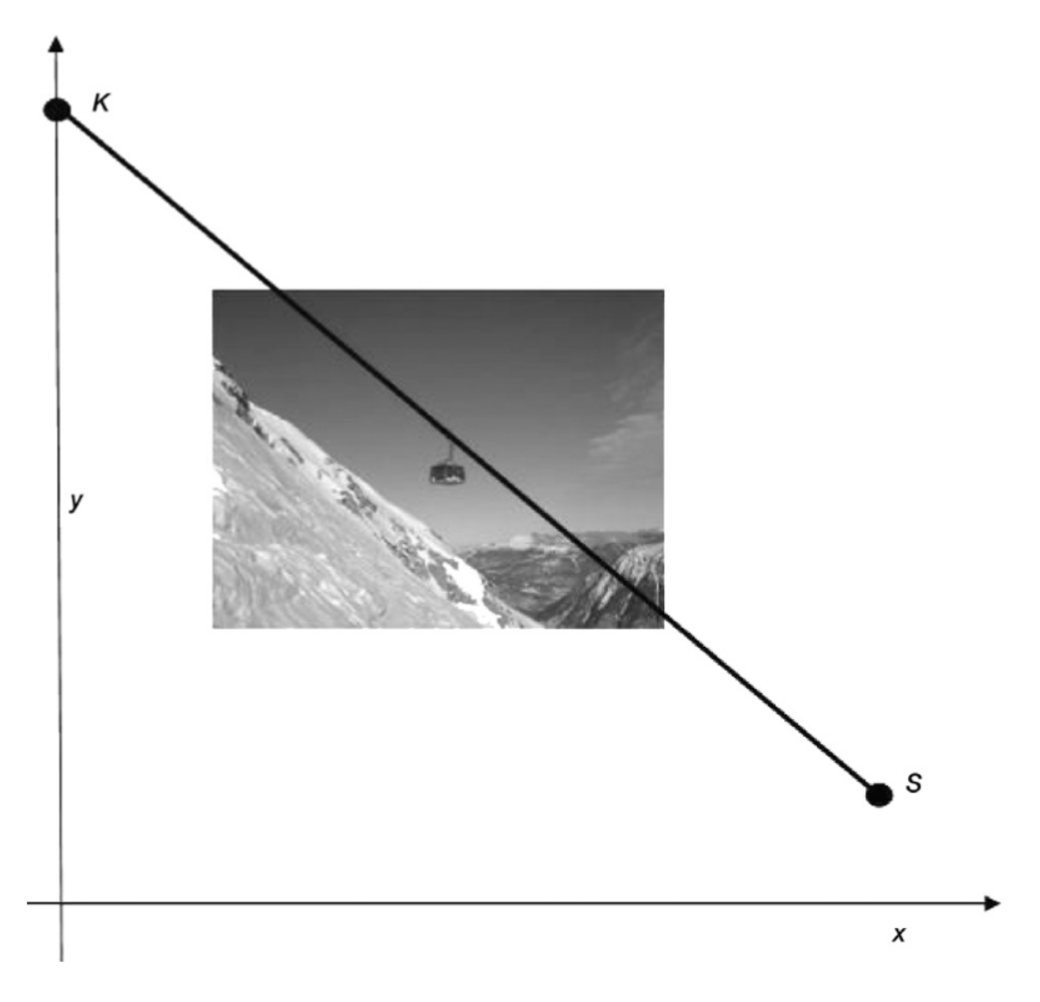
\includegraphics{../Bilder/Bild41-1.eps}}
	\end{center}
	
	Nach dieser Modellierung gilt: $K=(0|2\,100)$ und $S=(2\,160|1\,350)$
	
	\fbox{A} Bestimme den Steigungswinkel des Tragseils!
	
	An welcher Stelle gleicher Seeh�he wie $S$ m�sste die Talstation $S'$ stehen, wenn das Tragseil mit $100\,\%$ Steigung verlaufen soll?
	
	Gib die Koordinaten von $S'$ an!
	
		\item Mit zunehmender H�he nimmt der Luftdruck exponentiell ab. Dabei gilt f�r die H�he $h$ (gemessen in m �ber dem Meeresspiegel) und den Luftdruck $p$ (gemessen in mbar) n�herungsweise der folgende funktionale Zusammenhang: $p(h)=1\,013,25\cdot e^{-0,000118\cdot h}$.
		
		Berechne die prozentuelle Druckabnahme auf der Fahrt von der Sch�nbergalm (Seeh�he $1\,350$\,m) bis zur Bergstation Krippenstein (Seeh�he 2\,100\,m)!
		
		Kreuze die zutreffende(n) Aussage(n) an!
		
		\multiplechoice[5]{  %Anzahl der Antwortmoeglichkeiten, Standard: 5
						L1={Die prozentuelle Druckabnahme pro H�henmeter ist konstant.},   %1. Antwortmoeglichkeit 
						L2={Bei einer Verdopplung der H�he halbiert sich der Luftdruck.},   %2. Antwortmoeglichkeit
						L3={Die absolute Druckabnahme pro H�henmeter ist konstant.},   %3. Antwortmoeglichkeit
						L4={Der zur Funktion $p$ geh�rige Graph ist streng monoton fallend.},   %4. Antwortmoeglichkeit
						L5={Der zur Funktion $p$ geh�rige Graph n�hert sich asymptotisch der waagrechten Achse.},	 %5. Antwortmoeglichkeit
						L6={},	 %6. Antwortmoeglichkeit
						L7={},	 %7. Antwortmoeglichkeit
						L8={},	 %8. Antwortmoeglichkeit
						L9={},	 %9. Antwortmoeglichkeit
						%% LOESUNG: %%
						A1=1,  % 1. Antwort
						A2=4,	 % 2. Antwort
						A3=5,  % 3. Antwort
						A4=0,  % 4. Antwort
						A5=0,  % 5. Antwort
						}
						\end{enumerate}\leer
				
\antwort{
\begin{enumerate}
	\item \subsection{L�sungserwartung:} 
	
		$\tan(\alpha)=\frac{750}{2\,160}\Rightarrow\alpha\approx 19,15^\circ$ bzw. $\alpha\approx 0,3342$\,rad
		
		$S'=(750|1\,350)$
	 	
	\subsection{L�sungsschl�ssel:}
	\begin{itemize}
		\item  Ein Ausgleichspunkt f�r die korrekte Berechnung.
		
		L�sungsintervall: $[19^\circ;19,2^\circ]$ bzw. $[0,33\,\text{rad};0,335\,\text{rad}]$
		\item Ein Punkt f�r die korrekte Berechnung.
	\end{itemize}
	
	\item \subsection{L�sungserwartung:}
			
		$\dfrac{p(1\,350)-p(2\,100)}{p(1\,350)}\approx 0,085=8,5\,\%$
		
	\subsection{L�sungsschl�ssel:}
	
\begin{itemize}
	\item  Ein Punkt f�r eine korrekte Berechnung. L�sungsintervall $[0,084;0,085]$ bzw. $[8,4\,\%;8,5\,\%]$.
	
	L�sungen aus dem Intervall $[-0,085;-0,084]$ bzw. $[-8,5\,\%;-8,4\,\%]$ sind ebenso als richtig zu werten.
	\item  Multiple-Choice-Aufgabe: Ein Punkt ist genau dann zu geben, wenn ausschlie�lich alle laut L�sungserwartung richtigen Antwortm�glichkeiten angekreuzt sind.

\end{itemize}

\end{enumerate}}
		\end{langesbeispiel}